

\paragraph{} In this chapter we shall introduce and detail a prototype implementation of a modular, SGX-protected \textit{reference monitor} --- \textsc{Citadel}. First, its necessity will be motivated, and the challenges faced discussed. Then, the three-part architecture will be explained, relating various design decisions to the DIFC model it provides. A discussion about the architecture's performance and effectiveness is provided in §~\ref{sec:eval}.

\section{Motivation}
\paragraph{} Since its introduction in a 1972 report from Anderson~\cite{reference-monitor}

\section{Challenges}

\section{A Symbiotic Tripartite Relationship}

\begin{figure}[]
    \centering
    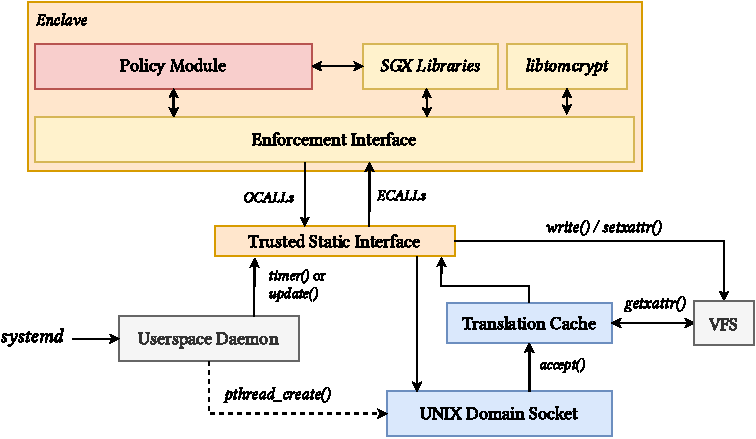
\includegraphics[width=\linewidth]{figures/EnclaveLayout.pdf}
    \caption{Abstract overview of an SGX enclave's protections.}
    \label{fig:sgx-basic}
\end{figure}